\documentclass[cal1spr16Lectures.tex]{subfiles}
%\AtBeginSubsection{
%	\begin{frame}[allowframebreaks]{}
%	\begin{multicols}{2}
%	\tableofcontents[currentsubsection]
%	\end{multicols}
%	\end{frame}
%	}
	
\begin{document}

%\section[Week 6]{Week 6: 22-26 February}

% % %
\subsubsection{\bf Wed 24 February}
\begin{frame}[allowframebreaks]{Wed 24 Feb}
\begin{itemize}\small
\item Exam 1: see the course webpage for the curve
\item MIDTERM 
\begin{itemize}\footnotesize
	\item Tuesday 8 March 6-7:30p
	\item If you have legitimate conflict, i.e., anything that is also scheduled in ISIS, I need to know now.  If you are not sure if it conflicts with a course, please have that instructor contact me ASAP.
	\item Cumulative.  Covers up to \S 3.9
	\item Morning Section: Walker rm 124
	
	Afternoon Section: Walker rm 218
\end{itemize}
\framebreak
\item Sub on Friday 26 Feb and Monday 29 Feb.
\item Possible sub on Wednesday 2 Mar.
\item Exam 2: Friday 4 March.  Covers up to \S 3.8.
\item Quizzes: Only some of the quiz problems are graded now.
\end{itemize}
\end{frame}

% % %
\subsection[3.5 Derivatives of Trigonometric Functions]{\S 3.5 Derivatives of Trigonometric Functions}
% % %

% % %
\begin{frame}{\S 3.5 Derivatives of Trigonometric Functions}
Trig functions are commonly used to model cyclic or periodic behavior in everyday settings.  Therefore it is important to know how these functions change across time.
\end{frame}

\begin{frame}{}{}
{\bf Fact:} Derivative formulas for sine and cosine can be derived using the following limits:
\begin{itemize}
	\item $\lim_{x \to 0} \frac{\sin x}{x}=1$
	\item $\lim_{x \to 0} \frac{\cos x -1}{x}=0$
\end{itemize}
(We will prove these limits in Chapter 4.)
\end{frame}

% % %
\begin{frame}
\begin{exe} Evaluate $\displaystyle\lim_{x \to 0} \frac{\sin 9x}{x}$ and $\displaystyle\lim_{x \to 0} \frac{\sin 9x}{\sin 5x}.$ \end{exe}
\end{frame}

% % %
\subsubsection{Derivatives of Sine and Cosine Functions}
% % %

% % %
\begin{frame}{\small Derivatives of Sine and Cosine Functions}
Using the previous limits and the definition of the derivative, we obtain
\begin{align*}
\frac{d}{dx} (\sin x) &= \cos x \\
\frac{d}{dx} (\cos x) &= -\sin x
\end{align*}
\end{frame}

% % %
\begin{frame}
Examining the graphs of sine and cosine illustrate the relationship between the functions and their derivatives.

\begin{center}
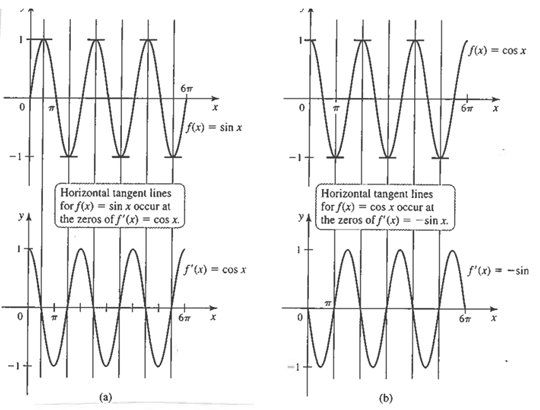
\includegraphics[scale=0.9]{pictures/Ch3sineCosine}
\end{center}
\end{frame}

% % %
\subsubsection{Trig Identities You Should Know}
% % %

% % %
\begin{frame}{\small Trig Identities You Should Know}
\begin{columns}[T]
\begin{column}{.5\textwidth}
\begin{itemize}\footnotesize
	\item $\sin^2 x + \cos^2 x = 1$ \vspace{0.2cm}
	\item $\tan^2 x + 1 = \sec^2 x$ \vspace{0.2cm}
	\item $\sin 2x =2\sin x \cos x$ \vspace{0.2cm}
	\item $\cos 2x = 1-2\sin^2 x$ \vspace{0.2cm}
	\item $\cos^2 x = \frac{1+\cos 2x}{2}$ \vspace{0.1cm}
	\item $\sin^2 x = \frac{1-\cos 2x}{2}$ \vspace{0.2cm}
\end{itemize}
\end{column}
\begin{column}{.5\textwidth}
\begin{itemize}\footnotesize
	\item $\tan x = \frac{\sin x}{\cos x}$ \vspace{0.2cm}
	\item $\cot x = \frac{\cos x}{\sin x}$ \vspace{0.2cm}
	\item $\cot x = \frac{1}{\tan x}$ \vspace{0.2cm}
	\item $\sec x = \frac{1}{\cos x}$ \vspace{0.1cm}
	\item $\csc x = \frac{1}{\sin x}$ \vspace{0.2cm}
\end{itemize}
\end{column}
\end{columns}
\end{frame}

% % %
\subsubsection{Derivatives of Other Trig Functions}
% % %

% % %
\begin{frame}{\small Derivatives of Other Trig functions}\footnotesize
\begin{align*}
\frac{d}{dx}(\tan x)&=\frac{d}{dx} \left( \frac{\sin x}{\cos x}\right) \\
 &= \frac{\cos x \cos x - (-\sin x)\sin x }{\cos^2 x} \\
&= \frac{\cos^2 x + \sin^2 x}{\cos^2 x} \\
&= \frac{1}{\cos^2 x} = \sec^2 x
\end{align*}
So \alert{$\frac{d}{dx} (\tan x)=\sec^2 x$}.
\end{frame}

% % %
\begin{frame}{}
By using trig identities and the Quotient Rule, we obtain
\begin{align*}
\alert{\frac{d}{dx} (\csc x)} &= \frac{d}{dx} \left( \frac{1}{\sin x}\right) = \alert{-\csc x \cot x} \\
\alert{\frac{d}{dx} (\sec x)} &= \frac{d}{dx} \left( \frac{1}{\cos x}\right) = \alert{\sec x \tan x} \\
\alert{\frac{d}{dx} (\cot x)} &= \frac{d}{dx} \left( \frac{1}{\tan x}\right) = \alert{-\csc^2 x}  
\end{align*}
\end{frame}

% % %
\begin{frame}
\begin{exe} Compute the derivative of the following functions:
\[f(x)=\frac{\tan x}{1+\tan x} \qquad g(x)=\sin x \cos x\]
\end{exe}
\end{frame}

% % %
\begin{frame}
\begin{exe} 
Use the difference and product rules to find the derivative of the function $y=\cos x-x\sin x$.
\begin{itemize}
\item[A. ] $-\sin x+x\cos x$
\item[B. ] $x\cos x$
\item[C. ] $-2\sin x-x\cos x$
\item[D. ] $x\cos x-2\sin x$
\end{itemize}
\end{exe}
\end{frame}

% % %
\subsubsection{Higher-Order Trig Derivatives}
% % %

% % %
\begin{frame}{\small Higher-Order Trig Derivatives}
There is a cyclic relationship between the higher order derivatives of $\sin x$ and $\cos x$:
\begin{columns}
\begin{column}{.45\textwidth}
\[\begin{split}
	f(x) &=\sin x \\  
	f^{\prime}(x) &=\cos x \\
	f^{\prime\prime}(x) &=-\sin x \\
	f^{(3)}(x) &=-\cos x \\
	f^{(4)}(x) &=\sin x 
\end{split}\]
\end{column}
\begin{column}{.6\textwidth}
\[\begin{split}
	g(x) &=\cos x \\
	g^{\prime}(x) &=-\sin x \\
	g^{\prime\prime}(x) &=-\cos x \\
	g^{(3)}(x) &=\sin x \\
	g^{(4)}(x) &=\cos x 
\end{split}\]
\end{column}
\end{columns}
\end{frame}

% % %
\subsubsection{Book Problems}
% % %

% % %
\begin{frame}
\begin{block}{3.5 Book Problems} 7-47 (odds), 57, 59, 61 \end{block} 
\end{frame}

% % %
\subsection[3.6 Derivatives as Rates of Change]{\S 3.6 Derivatives as Rates of Change}
% % %

% % %
\begin{frame}{\S 3.6 Derivatives as Rates of Change}
\begin{que}  
Why do we need derivatives in real life? 
\end{que}  

We look at four areas where the derivative assists us with determining the rate of change in various contexts.
\end{frame}

% % %
\subsubsection{Position and Velocity}
% % %

% % %
\begin{frame}{\small Position and Velocity}
Suppose an object moves along a straight line and its location at time $t$ is given by the position function $s=f(t)$.  The {\bf displacement} of the object between $t=a$ and $t=a+\Delta t$ is 
\[\Delta s = f(a+\Delta t)-f(a).\]
Here $\Delta t$ represents how much time has elapsed.
\end{frame}

% % %
\begin{frame}{}
We now define average velocity as 
\[\frac{\Delta s}{\Delta t}=\frac{f(a+\Delta t)-f(a)}{\Delta t}.\]
Recall that the limit of the average velocities as the time interval approaches 0 was the instantaneous velocity (which we denote here by $v$).  Therefore, the instantaneous velocity at $a$ is 
\[v(a)=\lim_{\Delta t \to 0} \frac{f(a+\Delta t)-f(a)}{\Delta t} = f^{\prime}(a).\]
\end{frame}

% % %
\subsubsection{Speed and Acceleration}
% % %

% % %
\begin{frame}{\small Speed and Acceleration}
In mathematics, speed and velocity are related but not the same -- if the \alert{velocity} of an object at any time $t$ is given by $v(t)$, then the \alert{speed} of the object at any time $t$ is given by 
\[|v(t)|=|f^{\prime}(t)|.\]
\end{frame}

% % %
\begin{frame}[allowframebreaks]{}
By definition, acceleration (denoted by $a$) is the instantaneous rate of change of the velocity of an object at time $t$.  Therefore,
\[a(t)=v^{\prime}(t)\]
and since velocity was the derivative of the position function $s=f(t)$, then 
\[a(t)=v^{\prime}(t)=f^{\prime\prime}(t).\]

\framebreak
{\bf Summary:}  Given the position function $s=f(t)$, the velocity at time $t$ is the first derivative, the speed at time $t$ is the absolute value of the first derivative, and the acceleration at time $t$ is the second derivative.
\end{frame}

% % %
\begin{frame}
\begin{que} Given the position function $s=f(t)$ of an object launched into the air, how would you know:
\begin{itemize}
	\item The highest point the object reaches?
	\item How long it takes to hit the ground?
	\item The speed at which the object hits the ground?
\end{itemize}
\end{que}
\end{frame}

% % %
\begin{frame}
\begin{exe}
A rock is dropped off a bridge and its distance $s$ (in feet) from the bridge after $t$ seconds is $s(t)=16t^2+4t$.  At $t=2$ what are, respectively, the velocity of the rock and the acceleration of the rock? 
\begin{itemize}
\item[A. ] $64$ ft/s; $16$ ft/s$^2$
\item[B. ] $68$ ft/s; $32$ ft/s$^2$
\item[C. ] $64$ ft/s; $32$ ft/s$^2$
\item[D. ] $68$ ft/s; $16$ ft/s$^2$
\end{itemize}
\end{exe}
\end{frame}

% % %
\subsubsection{Growth Models}
% % %

% % %
\begin{frame}{\small Growth Models}
Suppose $p=f(t)$ is a function of the growth of some quantity of interest.  The average growth rate of $p$ between times $t=a$ and a later time $t=a+\Delta t$ is the change in $p$ divided by the elapsed time $\Delta t$:
\[\frac{\Delta p}{\Delta t}=\frac{f(a+\Delta t)-f(a)}{\Delta t}.\]
\end{frame}

% % %
\begin{frame}{}
As $\Delta t$ approaches 0, the average growth rate approaches the derivative $\textstyle\frac{dp}{dt}$, which is the instantaneous growth rate (or just simply the growth rate).  Therefore,
\[\frac{dp}{dt}=\lim_{\Delta t \to 0} \frac{f(a+\Delta t)-f(a)}{\Delta t} = \lim_{\Delta t \to 0} \frac{\Delta p}{\Delta t}.\]
\end{frame}

% % %
\begin{frame}
\begin{exe} The population of the state of Georgia (in thousands) from 1995 ($t=0$) to 2005 ($t=10$) is modeled by the polynomial 
\[p(t)=-0.27t^2+101t+7055.\]
\begin{itemize}
	\item[(a)] What was the average growth rate from 1995 to 2005?
	\item[(b)] What was the growth rate for Georgia in 1997?
	\item[(c)] What can you say about the population growth rate in Georgia between 1995 and 2005?
\end{itemize}
\end{exe}
\end{frame}

% % %
\subsubsection{Average and Marginal Cost}
% % %

% % %
\begin{frame}{\small Average and Marginal Cost}
Suppose a company produces a large amount of a particular quantity.  Associated with manufacturing the quantity is a {\bf cost function} $C(x)$ that gives the cost of manufacturing $x$ items.  This cost may include a {\bf fixed cost} to get started as well as a {\bf unit cost} (or {\bf variable cost}) in producing one item.
\end{frame}

% % %
\begin{frame}{}
If a company produces $x$ items at a cost of $C(x)$, then the average cost is $\textstyle\frac{C(x)}{x}.$  This average cost indicates the cost of items already produced.  Having produced $x$ items, the cost of producing another $\Delta x$ items is $C(x+\Delta x)-C(x)$.  So the average cost of producing these extra $\Delta x$ items is 
\[\frac{\Delta C}{\Delta x}=\frac{C(x+\Delta x)-C(x)}{\Delta x}.\]
\end{frame}

% % %
\begin{frame}{}
If we let $\Delta x$ approach 0, we have
\[\lim_{\Delta x \to 0}\frac{\Delta C}{\Delta x}=C^{\prime}(x)\]
which is called the {\bf marginal cost}.  The marginal cost is the approximate cost to produce one additional item after producing $x$ items.

\vspace{1pc}
{\bf Note:}  In reality, we can't let $\Delta x$ approach 0 because $\Delta x$ represents whole numbers of items.
\end{frame}

% % %
\begin{frame}
\begin{exe} If the cost of producing $x$ items is given by 
\[C(x)=-0.04x^2+100x+800\]
for $0 \le x \le 1000$, find the average cost and marginal cost functions.  Also, determine the average and marginal cost when $x=500.$ \end{exe}
\end{frame}

% % %
\subsubsection{Book Problems}
% % %

% % %
\begin{frame}
\begin{block}{3.6 Book Problems} 9-19, 21-24, 30-33 (odds) \end{block}
\end{frame}

\end{document}